%\documentclass[conference]{IEEEtran}
%\IEEEoverridecommandlockouts
\documentclass{article}
\usepackage[utf8]{inputenc}
\usepackage[%
    left=1.0in,%
    right=1.0in,%
    top=1.0in,%
    bottom=1.0in,%
    paperheight=11in,%
    paperwidth=8.5in%
]{geometry}

% =======================
\usepackage{xeCJK}
\usepackage{amssymb}
\usepackage{amsmath}
\usepackage{amstext}
\usepackage{amsopn}
%\usepackage{algorithmic}
\usepackage{graphicx}
\usepackage{textcomp}
\usepackage{xcolor}

\usepackage{textcomp}

\usepackage{boxedminipage}
\usepackage{enumerate}
\usepackage{multirow}
\usepackage{url}
\usepackage{times}
\usepackage{version}
% \usepackage[pdftex]{graphicx}
\usepackage{epsfig}
\usepackage{epsf}
%\usepackage{graphics}
\usepackage{caption}
\usepackage{subfigure}
\usepackage{algorithm}
\usepackage{algpseudocode}
%\PassOptionsToPackage{bookmarks={false}}{hyperref}
%%%%%%%%%%%%
\usepackage{comment}
\usepackage{multicol}
\usepackage{booktabs}
\usepackage{dblfloatfix}
% ==========================

\setCJKmainfont[Path=fonts/]{msjh.ttc} % 中文字型
\setCJKmonofont[Path=fonts/]{msjh.ttc} % 中文等寬字型

\begin{document}

\title{E-Healthcare Management System}
\author{
  Cheng-Han Hsieh, 謝承翰\\
  \texttt{B103040012}
  \and
  Shih Yu Sun, 孫世諭\\
  \texttt{B103040001}
  \and
  Casper Liu, 劉世文\\
  \texttt{B093040051}
  \and
  Tina Tsou, 鄒宜庭\\
  \texttt{B096060032}
  \and
  Chia-Yen Huang, 黃嘉彥\\
  \texttt{B103040051}
  \and
  Ting-Hao Hsu, 許廷豪\\
  \texttt{B103040008}
}

\maketitle

\section{Outline}
\label{sec:outline}

\begin{figure}[h]
  \centering
  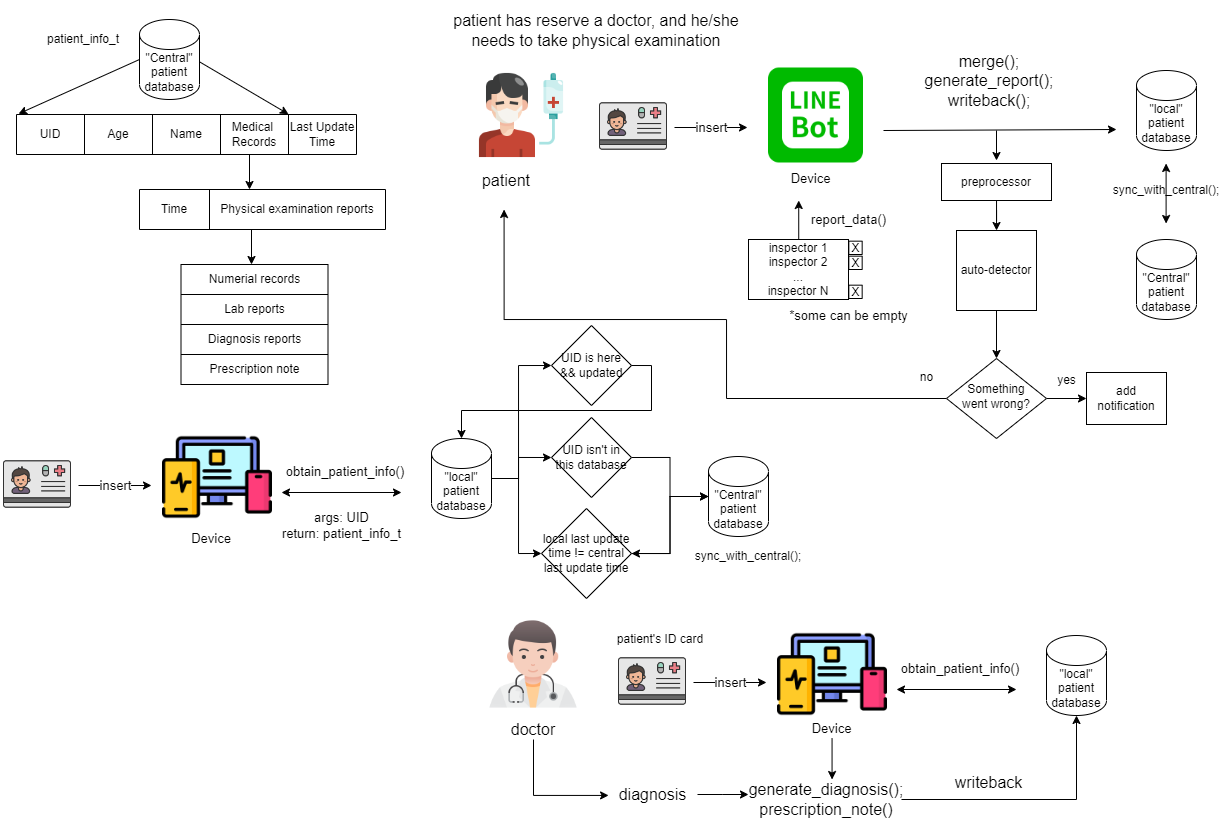
\includegraphics[scale = 0.3]{asset/flowchart.png}
  \caption{A simple example of outline.}
  \label{fig:flowchart}
\end{figure}


\section{Features}
\label{sec:features}

With this E-healthcare management system, the hospital/clinic can easily 
sync the information of patients with other health systems, manage 
the information of patients.
For patients, the patient can do most of the things online, for example, 
make a doctor appointment, look up the medical records and prescriptions, 
and obtain the physical reports at home. Even more, the system use machine 
learning to detect the abnormal data in the reports, notify the patient 
to prevent the disease becoming worse. 
To conclusion, the major features of the system can be summarized as 
followings: 
\begin{itemize}
  \item Automatically sync the information of patients between different health systems by using local and central database. 
  \item Facilitate the accessing of medical records and prescriptions, for both doctors and patients. 
  \item Introduce the automatic disease detecters by leveraging machine learning and big data. 
\end{itemize}

\section{Methodology}
\label{sec:methodology}
\subsection*{Database}
\begin{figure}[h]
  \centering
  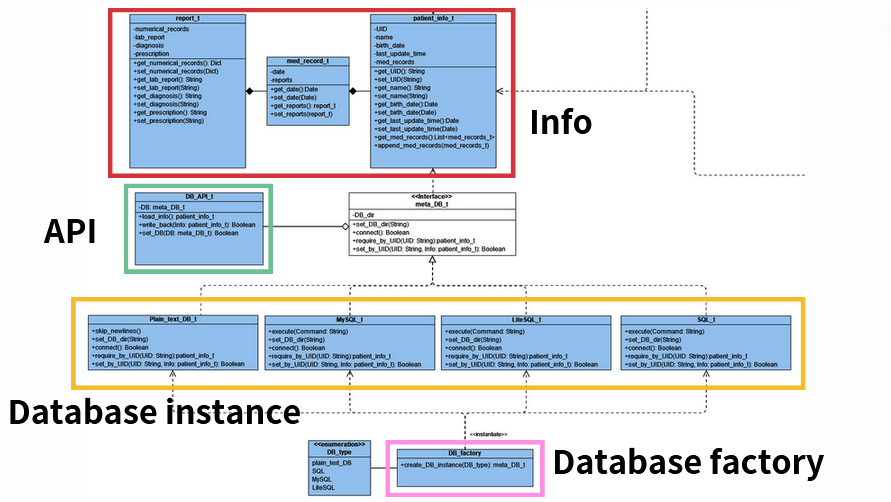
\includegraphics[scale = 0.7]{asset/DB_UML.png}
  \caption{The UML of the whole database.}
  \label{fig:DB_UML}
\end{figure}
\begin{figure}[h]
  \centering
  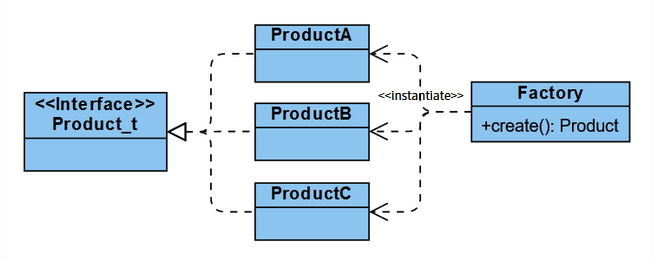
\includegraphics[scale = 0.7]{asset/simple_factory.png}
  \caption{The UML of a simple factory.}
  \label{fig:simple_factory}
\end{figure}

\section{Code}
\label{sec:code}

\section{Conclusion}
\label{sec:conclusion}

\section{Contribution}
\label{sec:contribution}

\end{document}